% =====================================================================
%  FoodYou -- Disruption Conformance Campaign
%  Results presentation. Overleaf-ready: pdflatex twice.
%
%  PLACEHOLDERS are marked \PENDING{...}. Two remain:
%    * storage_media results (run in progress)
%    * the six re-run cases (Section~\ref{sec:toolingrerun})
%  Search for \PENDING to find every one.
% =====================================================================
\documentclass[11pt,a4paper]{article}

\usepackage[utf8]{inputenc}
\usepackage[T1]{fontenc}
\usepackage[margin=2.4cm]{geometry}
\usepackage{booktabs}
\usepackage{graphicx}
\usepackage{xcolor}
\usepackage{listings}
\usepackage{caption}
\usepackage{tikz}
\usetikzlibrary{arrows.meta,positioning,fit,calc,backgrounds}
\usepackage[hidelinks]{hyperref}

\definecolor{accent}{RGB}{0,90,160}
\definecolor{warn}{RGB}{176,60,20}
\definecolor{good}{RGB}{20,110,60}
\definecolor{codebg}{gray}{0.96}

\lstset{basicstyle=\ttfamily\footnotesize, backgroundcolor=\color{codebg},
        frame=single, rulecolor=\color{gray!40}, breaklines=true,
        columns=fullflexible, framexleftmargin=4pt}

% Every unfinished figure is marked, so none can be forgotten.
\newcommand{\PENDING}[1]{\textcolor{warn}{\textbf{[PENDING: #1]}}}
\newcommand{\gate}[1]{\texttt{\small #1}}

\title{\vspace{-1.5em}\textbf{Disruption Conformance Testing of a Local-First
Mobile Application}\\[0.3em]
\large Results of a hybrid-\textbf{ioco} campaign over 748 generated test cases}
\author{}
\date{Campaign closed August 2026}

\begin{document}
\maketitle
\vspace{-2.5em}

% =====================================================================
\section{What was tested}
% =====================================================================

The subject is \textbf{FoodYou} (\texttt{com.maksimowiczm.foodyou}), a
local-first Android nutrition tracker written in Kotlin and Jetpack Compose. Its
entire state lives in an on-device Room/SQLite database; there is no server.

A formal specification (LNT), a System Interface describing how each abstract
gate is realised in the user interface, and an interpretation of the abstract
domain are composed and passed to CADP/TESTOR, which generates controllable test
cases. A concretization layer walks each test case against the running
application, applies disruptions, and returns an \textbf{ioco} verdict.

Nine test purposes were generated, yielding \textbf{793 test cases}; \textbf{748}
were executed. One purpose (\gate{extapi\_fail}) could not be run: its
disruption \emph{is} the loss of network connectivity, and the test device had no
route to the external catalogue for the duration of the campaign.

\medskip
\noindent\textbf{Conformance is relative to the specification.} Throughout this
report, a \textsc{fail} means the application produced an output the
specification forbids after a given trace. Whether the specification is itself a
faithful account of the world is a separate question, treated in
Section~\ref{sec:threats}.

% =====================================================================
\section{Verdicts and what they mean here}
% =====================================================================

\begin{figure}[h]
\centering
\begin{tikzpicture}[font=\footnotesize, node distance=6mm,
  dec/.style={draw, diamond, aspect=2.6, inner sep=1pt, align=center, fill=gray!8},
  end/.style={draw, rounded corners=3pt, minimum height=7mm, align=center},
  ar/.style={-{Stealth[length=2mm]}, thick, gray!70}]
\node[dec] (d1) {tester applied\\its stimulus?};
\node[end, fill=accent!12, right=20mm of d1] (inc) {\textsc{inconclusive}};
\node[dec, below=9mm of d1] (d2) {application\\responded?};
\node[dec, below=9mm of d2] (d3) {response permitted\\by the specification?};
\node[end, fill=good!12, right=20mm of d3] (pass) {\textsc{pass}};
\node[end, fill=warn!12, below=9mm of d3] (fail) {\textsc{fail}};
\draw[ar] (d1) -- node[above]{no} (inc);
\draw[ar] (d1) -- node[left]{yes} (d2);
\draw[ar] (d2) -- node[left]{yes} (d3);
\draw[ar] (d2.east) -| node[pos=0.25,below]{no (silent)} (inc.south);
\draw[ar] (d3) -- node[above]{yes} (pass);
\draw[ar] (d3) -- node[left]{no} (fail);
\end{tikzpicture}
\caption{The verdict procedure. \textsc{fail} is the last branch, not the
default: a stimulus that could not be applied yields no observation, so there is
nothing for the oracle to judge.}
\label{fig:verdict}
\end{figure}

\noindent\textbf{\textsc{pass}} --- the application responded, and the response is
one the specification permits.

\noindent\textbf{\textsc{fail}} --- the application responded with something the
specification forbids. This is a conformance counter-example \emph{with respect
to the specification}.

\noindent\textbf{\textsc{inconclusive}} --- the tester could not apply its
stimulus, or the disruption's own precondition was absent. No observation reached
the oracle, so no claim about the application is available. Under \textbf{ioco} a
\textsc{fail} must be \emph{earned}; an unappliable stimulus does not earn one.

\medskip
Runs in which the \emph{apparatus} failed --- the automation session died, the
device showed a system-level dialog, or the framework raised an exception ---
produce no verdict at all. They are neither \textsc{fail} nor
\textsc{inconclusive}, because both of those are statements about the
application. They are re-run, and Section~\ref{sec:toolingrerun} records what
they produced on re-execution.

% =====================================================================
\section{The nominal campaign}
% =====================================================================

The \gate{happy} purpose exercises the application with no disruption applied:
search the local catalogue, read a food's energy, log it to a meal, and read back
the daily total. It is the \textbf{control}. Its role is not to find defects but
to establish that a verdict under disruption can be attributed to the disruption
rather than to the tester or the environment.

\begin{table}[h]
\centering\small
\caption{Nominal campaign.}
\begin{tabular}{@{}lrrrr@{}}
\toprule
Purpose & Cases & \textsc{pass} & \textsc{inconc} & \textsc{fail} \\
\midrule
\gate{happy} & 104 & 90 & 13 & 1$^{\dagger}$ \\
\bottomrule
\end{tabular}
\end{table}

\noindent $^{\dagger}$ An apparatus failure, not a verdict; re-run in
Section~\ref{sec:toolingrerun}.

\noindent The 13 \textsc{inconclusive} cases all reach the external-catalogue
branch, where the fixture queries Open Food Facts for a product that catalogue
does not carry --- confirmed both by the application's own displayed source count
of~0 and by a direct query to the catalogue API. The tester cannot proceed, so no
observation is obtained. This is an honest coverage gap, discussed in
Section~\ref{sec:threats}.

Across the nominal campaign, \textbf{558} daily-total observations were checked
against the model's abstract value \emph{and} against an exact running sum of
what the tester had logged; \textbf{165} per-food energy readings were checked
against the application's own catalogue. None disagreed.

% =====================================================================
\section{The disruptions}
% =====================================================================

Eight disruptions were designed across four layers. Each is injected out of band
--- through SQL against the application's database, adb commands, or process
control --- never through the user interface, so the application cannot
distinguish the disruption from a genuine environmental failure.

Before any verdict was recorded, every injection was verified to \emph{bite} and
to \emph{let go}: its effect was confirmed on the device independently of the
application, and the device was confirmed to return to its prior state. A
disruption that does not manifest would yield a \textsc{pass} meaning only that
the application was never disturbed.

\begin{table}[h]
\centering\footnotesize
\caption{The eight disruptions, what each means for this application, and the
observable the specification demands in response.}
\label{tab:disruptions}
\begin{tabular}{@{}llp{4.6cm}p{4.4cm}@{}}
\toprule
Layer & Disruption & Meaning for FoodYou & Specification demands \\
\midrule
User/Env & \gate{UE1\_KILL} & The process is killed while a diary write is in
flight, then relaunched. & The write is rolled back and the daily total is
unchanged. \\
\addlinespace
User/Env & \gate{INPUT\_INVALID} & The user submits an invalid quantity. Carried
as a parameter rather than injected: the tester performs it as a user would. &
The entry is rejected and the daily total is unchanged. \\
\addlinespace
App & \gate{EXTAPI\_FAIL} & The remote catalogue is unreachable during an
external search. & A warning is surfaced; nutrition data is not invented. \\
\addlinespace
App & \gate{CACHE\_STALE} & A cached nutrition value has drifted from the
catalogue. & The authoritative value is returned, not the cached one. \\
\addlinespace
Database & \gate{DISRUPTION\_DB} & The write transaction aborts. & The failure is
reported and the daily total is unchanged. \\
\addlinespace
Database & \gate{DB\_CORRUPT} & A stored record is missing a required field. &
The corruption is detected and surfaced, not rendered as data. \\
\addlinespace
Infra & \gate{STORAGE\_FULL} & The write fails for lack of storage. & The failure
is reported and the daily total is unchanged. \\
\addlinespace
Infra & \gate{STORAGE\_MEDIA} & The storage medium errors on read. & A storage
error is surfaced, not a wrong entry and not silence. \\
\bottomrule
\end{tabular}
\end{table}

% =====================================================================
\section{Results by test purpose}
\label{sec:results}
% =====================================================================

\begin{table}[h]
\centering\small
\caption{Verdicts per test purpose. Percentages are of executed cases.}
\label{tab:results}
\begin{tabular}{@{}lrrrr@{}}
\toprule
Purpose & Cases & \textsc{pass} & \textsc{inconc} & \textsc{fail} \\
\midrule
\gate{happy}          & 104 & 90 & 13 & 1$^{\dagger}$ \\
\gate{input\_invalid} &  86 & 73 & 13 & 0 \\
\gate{cache\_stale}   &  48 & 42 &  6 & 0 \\
\gate{db\_corrupt}    &  40 &  0 &  3 & 37 \\
\gate{ue1\_kill}      & 108 &  8 & 15 & 85 \\
\gate{disruption\_db} & 109 &  7 & 15 & 87 \\
\gate{storage\_full}  & 109 &  7 & 18 & 84 \\
\gate{storage\_media} & \PENDING{cases} & \PENDING{} & \PENDING{} & \PENDING{} \\
\gate{extapi\_fail}   & \multicolumn{4}{c}{not executed --- no network route to the external catalogue} \\
\midrule
\textbf{Total}        & \PENDING{total} & & & \\
\bottomrule
\end{tabular}
\end{table}

\noindent $^{\dagger}$ Apparatus failures, re-run in
Section~\ref{sec:toolingrerun}; the figures above are as originally recorded.

\subsection{\gate{input\_invalid} --- 73/86 pass, no failures}
The application rejects an invalid quantity by withdrawing its Save control
rather than by displaying an error message. The oracle therefore checks the
stronger property: that the daily total is unchanged, i.e.\ that \emph{nothing
was written} rather than that \emph{something was said}. No case disagreed. The
13 \textsc{inconclusive} cases are the external-catalogue branch.

\subsection{\gate{cache\_stale} --- 42/48 pass, no failures}
With the catalogue value altered underneath it, the application re-reads and
reports the current authoritative figure rather than a cached one. Every
observation agreed with the database to the calorie.

\subsection{\gate{db\_corrupt} --- 37 conformance counter-examples}
\label{sec:dbcorrupt}

\paragraph{The setup.}
One thing is broken deliberately: the food's energy value in the application's
database is set to \texttt{NULL}. The product no longer has a calorie figure.

\paragraph{What the tester did.}
Searched for the food, opened it, and saved it to a meal --- an ordinary add,
exactly as a user would perform it.

\paragraph{What the application did.}
\begin{enumerate}\setlength\itemsep{1pt}
  \item It \textbf{created the entry}. The food appears in the diary under
        Breakfast.
  \item It \textbf{detected that the record was incomplete} and labelled the
        entry \emph{``Food is missing required fields''}.
  \item It \textbf{declined to invent an energy}, displaying \texttt{---} rather
        than \texttt{0}.
  \item The daily total \textbf{remained at zero}.
\end{enumerate}

\paragraph{What the specification requires.}
After a valid add with no other disruption in the trace, exactly one output is
permitted:

\begin{center}
\gate{CONFIRM\_TOTAL (COMMITTED, bump(total), fid)}
\end{center}

\noindent The daily total must rise. The application left it unchanged, which the
specification forbids. All 37 failures carry this identical signature.

\paragraph{Why this is a defect and not a modelling artefact.}
The application did not refuse the entry --- it saved it. The entry is in the
diary. But the daily total, which the application computes from the entries in
that diary, does not include it. The application is therefore holding a saved
entry that its own arithmetic ignores, and the specification is right to forbid
that outcome.

\paragraph{What the campaign did \emph{not} see.}
The same screen also reports protein, fat and carbohydrate. From that same
incomplete record, the application counted \textbf{100\,g of fat}:

\begin{center}
\ttfamily
0 / 2000 kcal \quad---\quad ``2000 calories left'' \\
Fats \quad 100 / 67\,g \quad(over the goal)
\end{center}

\noindent The application refused the record's energy and accepted its fat. Same
record, two opposite decisions.

No \textbf{ioco} verdict could report this, because the specification describes
only the calorie total; the macronutrients are on the screen but not in the
model, so nothing was checking them. It was found by a separate check comparing
the application's calorie figure against its own macronutrient figures ---
100\,g of fat implies roughly 900\,kcal, and the screen read zero.
Section~\ref{sec:defect} treats this in full.

\medskip
\noindent\fbox{\begin{minipage}{0.95\textwidth}
In short: the application was told a record was incomplete, and then trusted half
of it --- refusing the calories, counting the fat, and reporting to the user that
they had consumed nothing.
\end{minipage}}

\subsection{\gate{ue1\_kill}, \gate{disruption\_db}, \gate{storage\_full} --- 256 conformance counter-examples}
\label{sec:writepath}

\paragraph{The setup.}
Three different things are broken, each aimed at the same promise --- \emph{a
write that fails leaves the daily total exactly as it was}:

\begin{itemize}\setlength\itemsep{1pt}
  \item \gate{UE1\_KILL}: the application's process is killed and relaunched.
  \item \gate{DISRUPTION\_DB}: a database trigger makes the insert raise and the
        transaction roll back.
  \item \gate{STORAGE\_FULL}: the device's storage is filled, so a write has
        nowhere to land.
\end{itemize}

\noindent These fail at three separate layers --- process, database, filesystem
--- so they exercise three independent implementation paths to one requirement.

\paragraph{What the tester did.}
Searched for the food, opened it, saved it to a meal, then read the daily total
back. An ordinary add, with the disruption applied.

\paragraph{What the specification requires.}
After any of the three, exactly one output is permitted:

\begin{center}
\gate{CONFIRM\_TOTAL (ROLLED\_BACK, total, fid)}
\end{center}

\noindent where \gate{total} is the value from \emph{before} the attempt. The
daily total must not move.

\paragraph{What the application did.}
The total rose. The entry was counted, and the application reported a figure that
included it --- an output the specification forbids after that trace. 256 cases
across the three purposes: 85, 87 and 84 respectively.

\paragraph{The passes are not evidence of correct behaviour.}
The three purposes recorded 8, 7 and 7 passes. \textbf{Every one of them observed
the same value}: a daily total already at \textsc{over}.

\textsc{over} is the saturating band --- the top of the scale. Once the total has
reached it, a further entry cannot change which band the total falls into,
whether the write landed or not. The abstraction is therefore unable to
distinguish the two outcomes, and the oracle records agreement because it cannot
observe disagreement.

\medskip
\noindent\fbox{\begin{minipage}{0.95\textwidth}
These 22 cases pass because the specification cannot express the difference at
that point, not because the application behaved as required. A saturating
abstraction makes its own requirement unfalsifiable above the saturation point.
\end{minipage}}

\medskip
\noindent The same limitation is what conceals the defect of
Section~\ref{sec:defect}: an abstraction chosen to describe a quantity coarsely
will not report a discrepancy finer than its own resolution.

\paragraph{Conditions.}
Section~\ref{sec:threats} records what is known about the point in the write
sequence at which these disruptions were applied.

\subsection{\gate{storage\_media}}
\PENDING{result, cause, and interpretation --- run in progress}

\subsection{\gate{extapi\_fail} --- not executed}
The disruption is the loss of connectivity to the external catalogue, and the
device had no route out for the duration of the campaign. Its injection could
therefore be neither applied nor verified, and its branch requires the external
catalogue to respond. Running it would have produced rows describing the test
host. It is excluded rather than reported.

% =====================================================================
\section{Apparatus failures and their re-execution}
\label{sec:toolingrerun}
% =====================================================================

Six runs failed because the testing apparatus failed, not the application. These
produce no verdict and are re-executed rather than counted.

\begin{table}[h]
\centering\footnotesize
\caption{Apparatus failures, their cause, and the verdict obtained on
re-execution.}
\begin{tabular}{@{}llll@{}}
\toprule
Purpose & Case & Cause & Verdict on re-run \\
\midrule
\gate{happy}          & v2  & unhandled framework exception & \PENDING{} \\
\gate{ue1\_kill}      & v53 & tester stimulus not applied   & \PENDING{} \\
\gate{disruption\_db} & v47 & tester stimulus not applied   & \PENDING{} \\
\gate{storage\_full}  & v11 & automation session died       & \PENDING{} \\
\gate{storage\_full}  & v17 & automation session died       & \PENDING{} \\
\gate{storage\_full}  & v48 & automation session died       & \PENDING{} \\
\gate{storage\_media} & \PENDING{} & \PENDING{} & \PENDING{} \\
\bottomrule
\end{tabular}
\end{table}

\noindent A separate incident is recorded for completeness. During the original
execution of \gate{storage\_media} the test device's operating system became
unresponsive and displayed a system-level dialog over the application. 138
consecutive cases then failed before reaching their disruption. The framework at
the time logged a warning and continued; it now refuses to start a test case
whose initial screen cannot be reached, and abandons a purpose after three
consecutive apparatus failures. The purpose was re-executed from a restored
device; Section~\ref{sec:results} reports that execution.

% =====================================================================
\section{A defect the specification could not express}
\label{sec:defect}
% =====================================================================

\begin{figure}[h]
\centering
\fbox{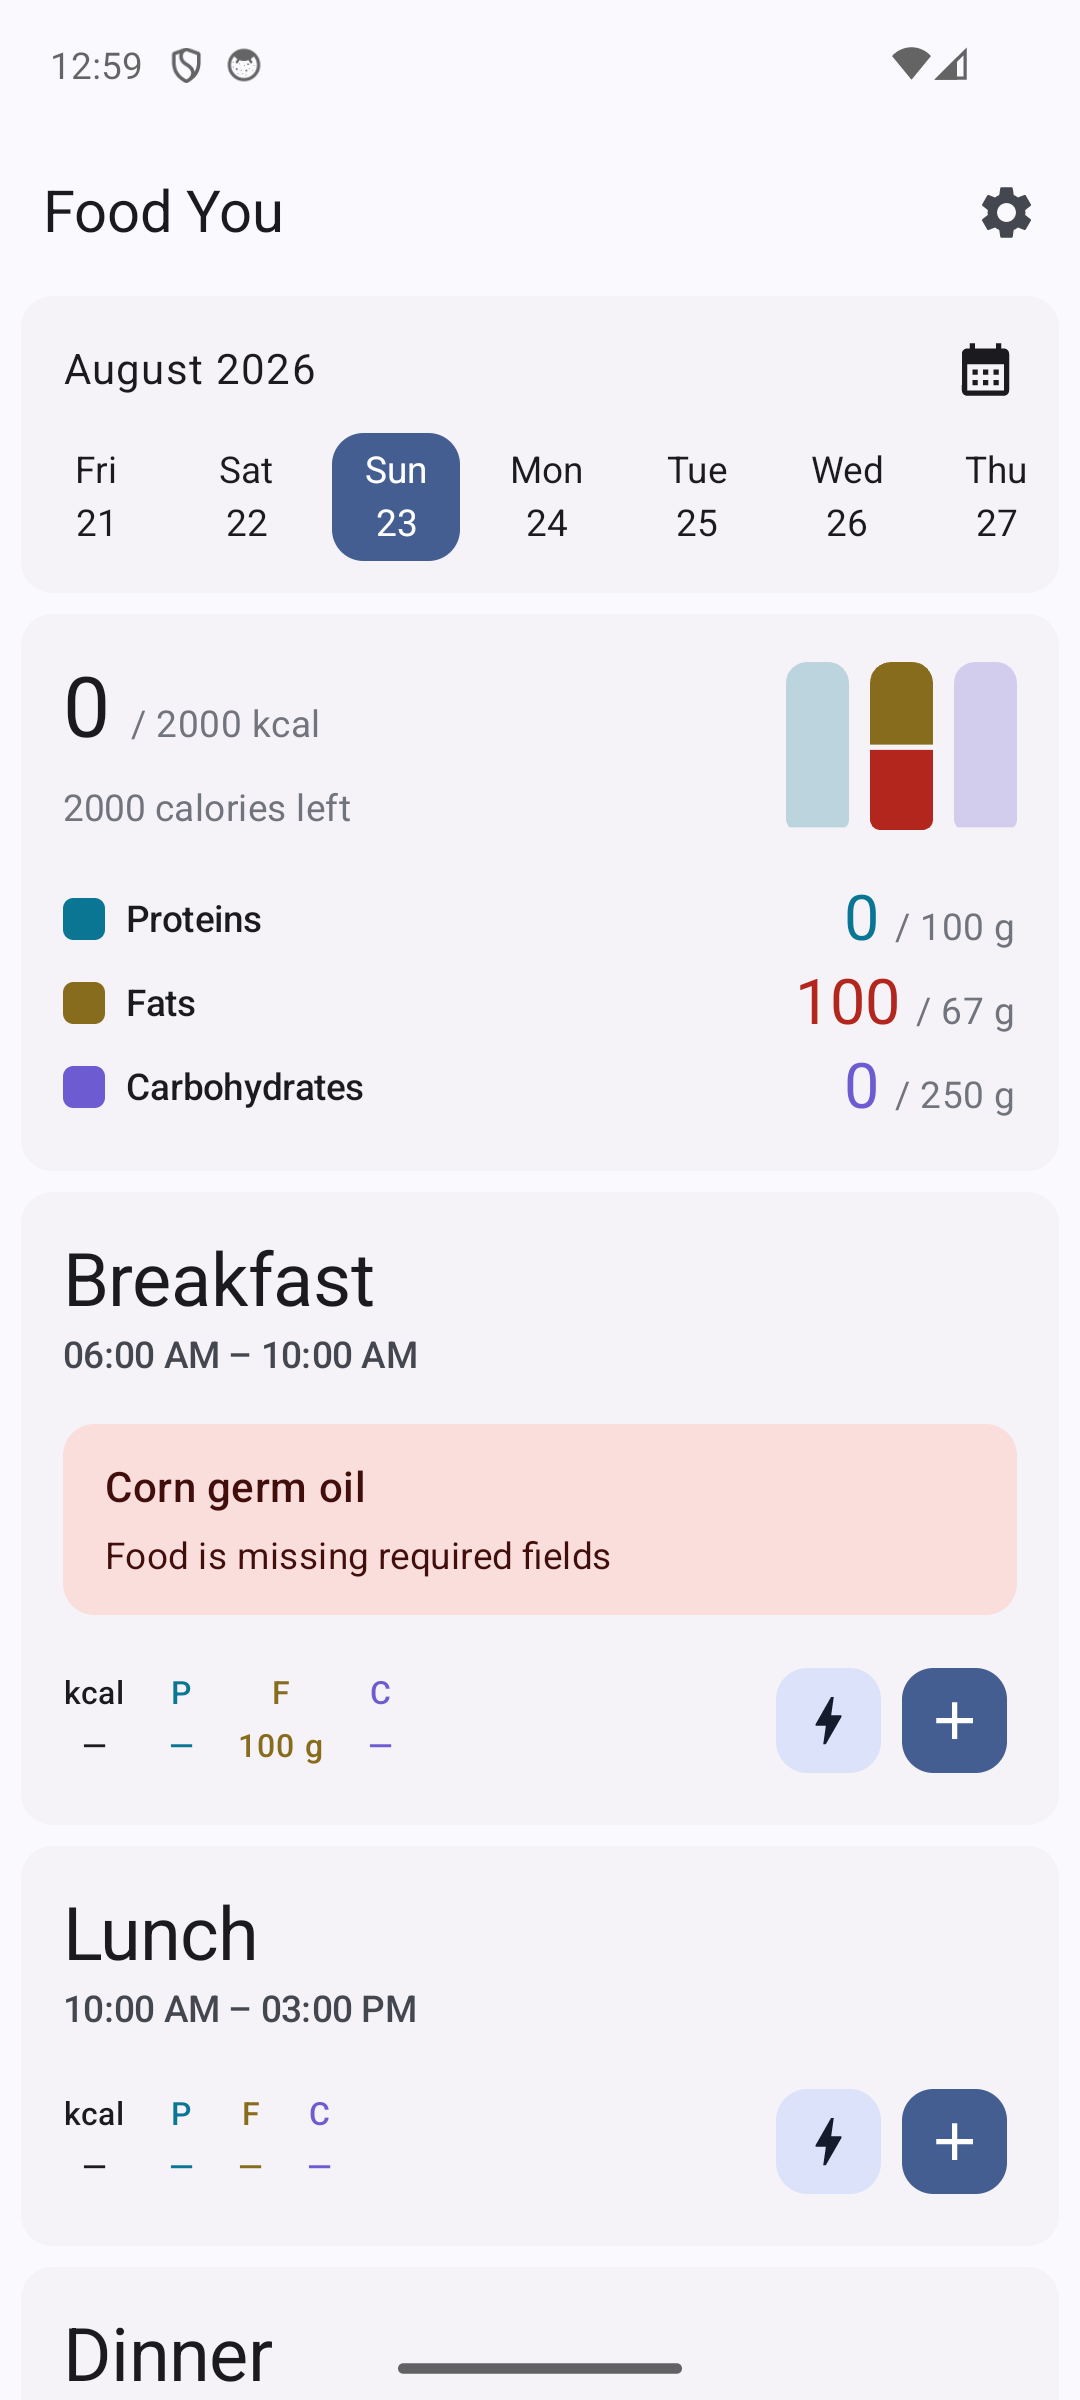
\includegraphics[width=0.42\textwidth]{figures/db_corrupt_evidence.png}}
\caption{The application under \gate{DB\_CORRUPT}. The entry is correctly flagged
\emph{``Food is missing required fields''} and its energy is withheld
(\texttt{kcal ---}); the same record's \textbf{100\,g of fat} is nonetheless
counted, and the header reports \textbf{``0 / 2000 kcal --- 2000 calories
left''}.}
\label{fig:defect}
\end{figure}

Under \gate{DB\_CORRUPT} the energy of the food under test is set to
\texttt{NULL} and 100\,g of a pure-fat product is logged. The application:

\begin{enumerate}\setlength\itemsep{1pt}
  \item \textbf{detects} the corruption and labels the entry \emph{``Food is
        missing required fields''};
  \item \textbf{declines to invent an energy}, displaying \texttt{---} rather
        than \texttt{0};
  \item \textbf{counts that same record's 100\,g of fat} into the daily total.
\end{enumerate}

The day header therefore reads \textbf{``0 / 2000 kcal --- 2000 calories left''}
beside \textbf{``Fats 100 / 67\,g''}, the latter over its goal. The application
trusts one field of a record it has itself declared untrustworthy, and a user who
has logged 100\,g of oil is told they have their entire daily allowance
remaining.

\subsection*{Why the test suite did not report it}

The failure this purpose \emph{did} report (Section~\ref{sec:dbcorrupt}) is
unrelated: the daily total not rising. The inconsistency above was invisible to
every \textbf{ioco} verdict, because \gate{DailyTotal} models energy alone. The
macronutrients are displayed on the same screen, computed by the same code from
the same rows, and the specification says nothing about them --- so nothing could
contradict.

It was caught by an oracle operating \emph{below} the abstraction: a check that
the energy the application displays is consistent with the macronutrients it
displays, using fixed conversion factors,
\[
\mathrm{kcal} \;\approx\; 4p + 9f + 4c .
\]
A day holding 100\,g of fat cannot also hold 0\,kcal. The check requires no
external reference --- it compares the application against itself --- and it
flagged this screen at a discrepancy of \textbf{900\,kcal}.

\subsection*{Why this is the campaign's most significant result}

It is a genuine defect, visible to a user, in the direction that matters for a
calorie tracker: the figure is wrong \emph{low}, and the application reports
confidence in it.

More importantly, it is evidence for a general claim. The abstraction --- a
saturating band over a single quantity --- is what limited the tool. The defect
was on screen, at a moment the tester had already stopped, in numbers the
application itself displayed, and it was missed because the specification
described only one of them.

\medskip
\noindent\fbox{\begin{minipage}{0.95\textwidth}
A concretization layer needs oracles of its own, not merely the enforcement of an
abstract specification. Checks that operate on concrete values the model does not
mention can detect defects the abstraction cannot express --- and are reported as
\emph{findings} rather than conformance verdicts, since they violate nothing the
specification asserts.
\end{minipage}}

\medskip
\noindent Making this a conformance counter-example rather than a finding requires
the macronutrients to enter the specification. That is future work.

% =====================================================================
\section{Threats to validity}
\label{sec:threats}
% =====================================================================

\paragraph{The specification's timing assumption.}
The three write-path disruptions require a rollback after an interrupted write.
The injections fire when the generated test case reaches the disruption gate,
which follows completion of the concrete steps for logging an entry. Whether the
write is durable before that point --- and therefore whether the specification's
antecedent holds as intended --- is not established by this campaign. The
verdicts stand with respect to the specification as written; a reader should know
the condition under which they were obtained.

\paragraph{Specification completeness.}
The specification does not describe logging a food whose record is incomplete
(Section~\ref{sec:dbcorrupt}), nor does it describe the macronutrients
(Section~\ref{sec:defect}). Both gaps were located by the campaign rather than
anticipated.

\paragraph{Coverage not achieved.}
Quantity was never varied: every entry uses the application's 100\,g default, so
all arithmetic checks ran on round numbers and rounding behaviour is untested.
Only one food was ever logged, so the abstraction's stated single-food validity
condition was never stressed. The external catalogue branch was never exercised.

\paragraph{Single execution.}
One repetition per test case. Stability was confirmed on a subset; no suite-wide
flakiness rate has been measured.

\paragraph{Test environment.}
One application, one device, one Android image. The device had no network route
for the duration, so no external-source verdict is available. The host was
memory-constrained and the emulator fell back to software rendering; on one
occasion the device's operating system became unresponsive
(Section~\ref{sec:toolingrerun}).

% =====================================================================
\section{Summary}
% =====================================================================

\PENDING{final counts, once storage\_media and the six re-runs are complete}

\begin{itemize}\setlength\itemsep{2pt}
  \item Every injection was verified to take effect on the device and to be
        reversed, independently of the application, before any verdict was
        recorded.
  \item \gate{input\_invalid} and \gate{cache\_stale} produced no failures: the
        application rejects invalid input without writing, and re-reads its
        catalogue rather than serving a stale value.
  \item \gate{db\_corrupt} produced 37 conformance counter-examples of a single
        signature: the application accepted an entry whose energy it could not
        determine, and left the daily total unchanged, where the specification
        requires it to rise.
  \item The three write-path disruptions produced 256 conformance
        counter-examples: the daily total rose where the specification requires
        it to remain unchanged.
  \item \textbf{293 conformance counter-examples in total}, across four of the
        eight disruptions.
  \item One genuine defect was found that no \textbf{ioco} verdict could express,
        by an oracle operating below the abstraction
        (Section~\ref{sec:defect}).
\end{itemize}

\end{document}
